% Intestazione
\fancyhead[L]{3 \hspace{0.2cm} Casi d'uso} % Testo a sinistra


\section{Casi d'uso}
\label{sec:casi_uso}

\subsection{Scopo}

Lo scopo di questa sezione è descrivere in maniera dettagliata i casi d’uso individuati dal
gruppo, in riferimento alle funzionalità dell’applicazione.


\subsection{Attori}
\label{sec:attori}

L’applicazione prevede la presenza di due \emph{Attori}\textsubscript{\textbf{\textit{G}}} principali:

\begin{itemize}
    \item \textbf{Utente}: Persona che utilizza l'applicazione interagendo direttamente con il sistema e avendo accesso a tutte le funzionalità del chatbot.
    \item \textbf{\emph{Scheduler}\textsubscript{\textbf{\textit{G}}}}: Lo \emph{Scheduler} è un sistema che si occupa di pianificare e gestire l'aggiornamento automatico periodico del \emph{database vettoriale}\textsubscript{\textbf{\textit{G}}}. Lo \emph{Scheduler} è fondamentale per mantenere il database aggiornato e garantire che il sistema abbia sempre a disposizione le informazioni più recenti e precise per rispondere alle domande degli utenti.

\end{itemize}


\subsection{Lista casi d'uso}




% TEMPLATE

\begin{comment}
\hypertarget{UC0}{}
\subsubsection{UC0: \dots}

\begin{figure}[h]
    \centering
    
\includegraphics[width=\textwidth]{placeholder.png}
    \caption{\dots}
\end{figure}

\begin{itemize}
    \item \textbf{Attori principali}: \dots;
    \item \textbf{Precondizioni}: \dots;
    % Oppure, se ci sono più precondizioni:
    \item \textbf{Precondizioni}: 
    \begin{itemize}
        \item \dots;
        \item \dots.
    \end{itemize}
    \item \textbf{Trigger}: \dots;
    \item \textbf{Postcondizioni}: \dots;
    \item \textbf{Scenario principale}:
    \begin{enumerate}
        \item \dots;
        \item \dots.
    \end{enumerate}
    \item \textbf{Sottocasi d'uso}:
    \begin{itemize}
        \item \dots;
        \item \dots.
    \end{itemize}
    \item \textbf{Scenario alternativo}:
    \begin{enumerate}
        \item \dots;
        \item \dots.
    \end{enumerate}
\end{itemize}
\end{comment}




\hypertarget{UC1}{}
\subsubsection{UC1: Inserimento di un'interrogazione in linguaggio naturale}

\begin{figure}[h]
    \centering
    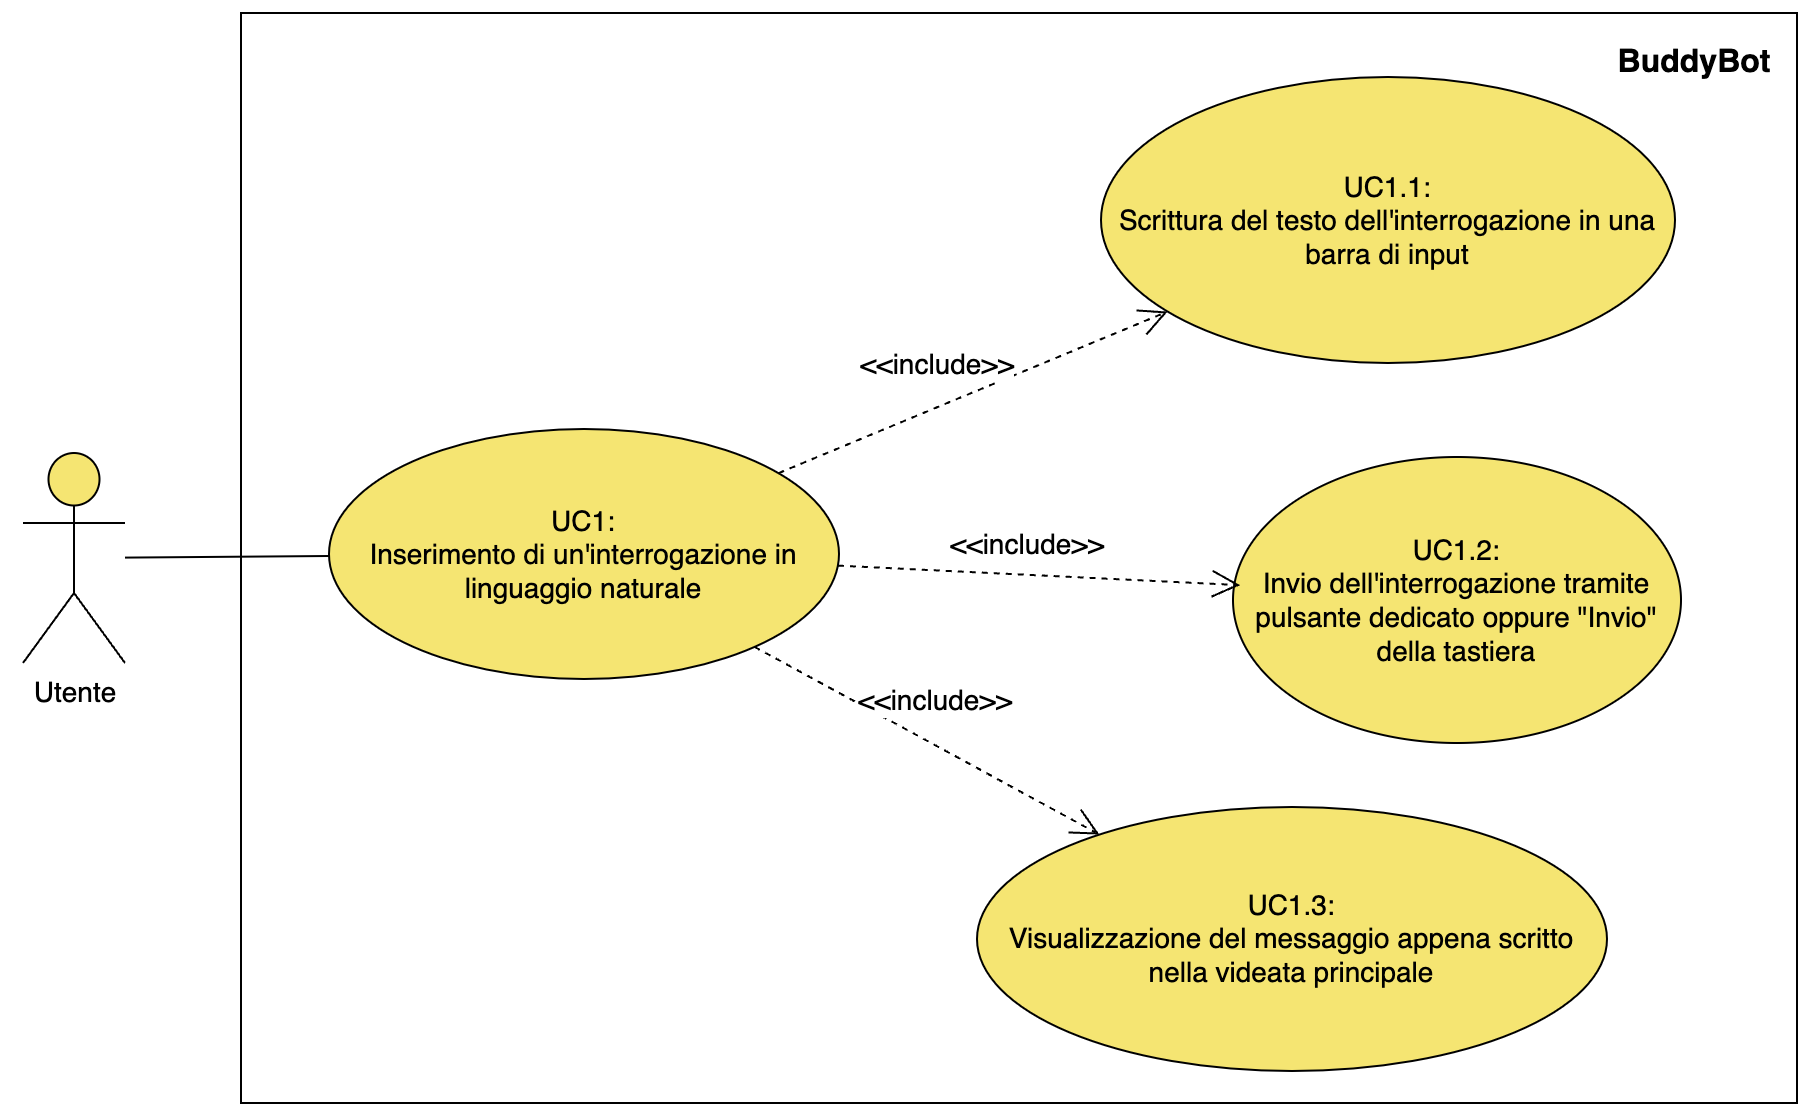
\includegraphics[width=\textwidth]{UC1.png}
    \caption{Inserimento di un'interrogazione in linguaggio naturale}
\end{figure}

\begin{itemize}
    \item \textbf{\emph{Attori} principali}: Utente;
    \item \textbf{Precondizioni}: L'utente deve avere accesso all'interfaccia dell'applicazione connessa al database;
    \item \textbf{\emph{Trigger}\textsubscript{\textbf{\textit{G}}}}: L'utente desidera inserire un'interrogazione in linguaggio naturale nella barra di input;
    \item \textbf{Postcondizioni}: L'interrogazione viene inserita e inviata.
    \item \textbf{\emph{Scenario principale}\textsubscript{\textbf{\textit{G}}}}:
    \begin{enumerate}
        \item L'utente accede all'interfaccia dell'applicazione;
        \item L'utente scrive l'interrogazione in linguaggio naturale nella barra di input.
        \item L'utente invia l'interrogazione tramite il pulsante dedicato o "Invio" dalla tastiera.
        \item \bulhyperlink{UC8.1}{UC8.1}: Il sistema mostra il messaggio generato nella schermata principale.
    \end{enumerate}
\end{itemize}

\newpage

\hypertarget{UC2}{}
\subsubsection{UC2: Visualizzazione della risposta generata}

\begin{figure}[h]
    \centering
    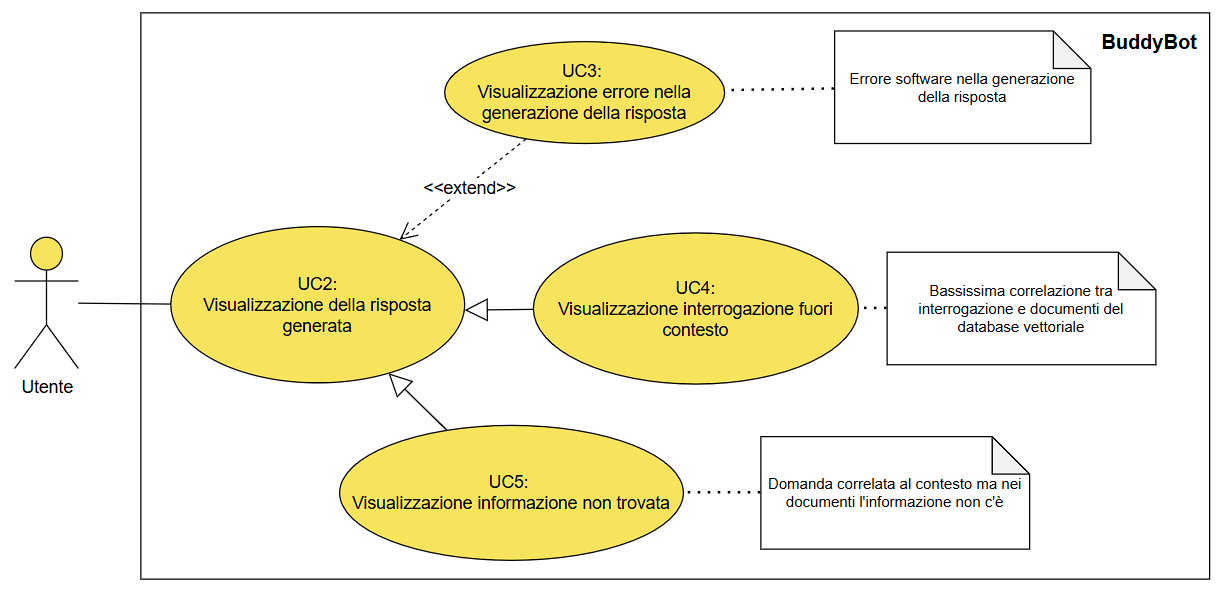
\includegraphics[width=\textwidth]{UC2+UC3+UC4+UC5.png}
    \caption{Visualizzazione della risposta generata}
\end{figure}

\begin{itemize}
    \item \textbf{Attori principali}: Utente;
    \item \textbf{Precondizioni}: Il sistema ha generato correttamente la risposta alla domanda dell'utente;
    \item \textbf{Trigger}: L'utente desidera visualizzare la risposta alla domanda che ha posto;
    \item \textbf{Postcondizioni}: L'utente visualizza la risposta generata dal sistema;
    \item \textbf{Scenario principale}:
    \begin{enumerate}
        \item Il sistema ha generato correttamente la risposta alla domanda dell'utente;
        \item L'utente visualizza la risposta generata dal sistema.
    \end{enumerate}
    \item \textbf{Scenario alternativo}:
    \begin{enumerate}
        \item \bulhyperlink{UC3}{UC3}: Visualizzazione errore nella generazione della risposta.
    \end{enumerate}
    \item \textbf{Casi che ereditano}:
    \begin{itemize}
        \item \bulhyperlink{UC4}{UC4}: Visualizzazione interrogazione fuori contesto;
        \item \bulhyperlink{UC5}{UC5}: Visualizzazione informazione non trovata.
    \end{itemize}
\end{itemize}

\hypertarget{UC3}{}
\subsubsection{UC3: Visualizzazione errore nella generazione della risposta}
\begin{itemize}
    \item \textbf{Attori principali}: Utente;
    \item \textbf{Precondizioni}: Il sistema non è riuscito a generare la risposta alla domanda dell'utente a causa di un errore interno;
    \item \textbf{Trigger}: L'utente desidera ricevere una risposta in linguaggio naturale alla domanda che ha posto;
    \item \textbf{Postcondizioni}: Viene visualizzato un messaggio di errore, chiedendo di riprovare più tardi;
    \item \textbf{Scenario principale}:
    \begin{enumerate}
        \item \bulhyperlink{UC1}{UC1}: L'utente inserisce un'interrogazione in linguaggio naturale;
        \item Si genera un errore durante il processamento della domanda che non permette la generazione della risposta;
        \item Viene visualizzato un messaggio di errore, chiedendo di riprovare più tardi.
    \end{enumerate}
\end{itemize}

\hypertarget{UC4}{}
\subsubsection{UC4: Visualizzazione interrogazione fuori contesto}
\begin{itemize}
    \item \textbf{Attori principali}: Utente;
    \item \textbf{Precondizioni}: Il sistema ha rilevato una bassissima correlazione tra l'interrogazione scritta dall'utente e i documenti del \emph{database vettoriale};
    \item \textbf{Trigger}: L'utente desidera visualizzare una risposta contenente informazioni legate esclusivamente ai contenuti del \emph{database vettoriale} associato al sistema;
    \item \textbf{Postcondizioni}: Viene visualizzato un messaggio che comunica all'utente che la domanda inserita è fuori contesto e che quindi è impossibile generare una risposta;
    \item \textbf{Scenario principale}:
    \begin{enumerate}
        \item \bulhyperlink{UC1}{UC1}: L'utente inserisce un'interrogazione in linguaggio naturale;
        \item Il sistema analizza la frase e cerca di contestualizzarla confrontandola con i dati presenti nel database;
        \item Il sistema rileva che la frase è fuori contesto e non può essere associata a nessuna informazione rilevante nel database;
        \item Il sistema invia un messaggio all'utente indicando che la domanda inserita è fuori contesto e richiede ulteriori chiarimenti.
    \end{enumerate}
    \item \textbf{Eredita da}:
    \begin{itemize}
        \item \bulhyperlink{UC2}{UC2}: Visualizzazione della risposta generata.
    \end{itemize}
\end{itemize}

\hypertarget{UC5}{}
\subsubsection{UC5: Visualizzazione errore informazione non trovata}
\begin{itemize}
    \item \textbf{Attori principali}: Utente;
    \item \textbf{Precondizioni}: Il sistema non ha trovato nei documenti di contesto l'informazione che l'utente ha domandato;
    \item \textbf{Trigger}: L'utente desidera visualizzare una risposta contenente le informazioni che ha richiesto nella domanda che ha posto al sistema;
    \item \textbf{Postcondizioni}: L'utente visualizza come risposta un messaggio del sistema in cui gli viene segnalata la mancanza dell'informazione 
    richiesta nei documenti individuati come contesto;
    \item \textbf{Scenario principale}:
    \begin{enumerate}
        \item Il sistema individua alcuni documenti di contesto nel \emph{database vettoriale} correlati alla domanda dell'utente;
        \item Il sistema non trova nei documenti di contesto l'informazione che l'utente ha domandato;
        \item L'utente visualizza come risposta un messaggio del sistema in cui gli viene segnalata la mancanza dell'informazione richiesta
        nei documenti individuati come contesto.
    \end{enumerate}
    \item \textbf{Eredita da}:
    \begin{itemize}
        \item \bulhyperlink{UC2}{UC2}: Visualizzazione della risposta generata.
    \end{itemize}
\end{itemize}

\newpage

\hypertarget{UC2.1}{}
\subsubsubsection{UC2.1: Visualizzazione dei file da cui il sistema ha preso i dati per la risposta alla domanda}

\begin{figure}[h]
    \centering
    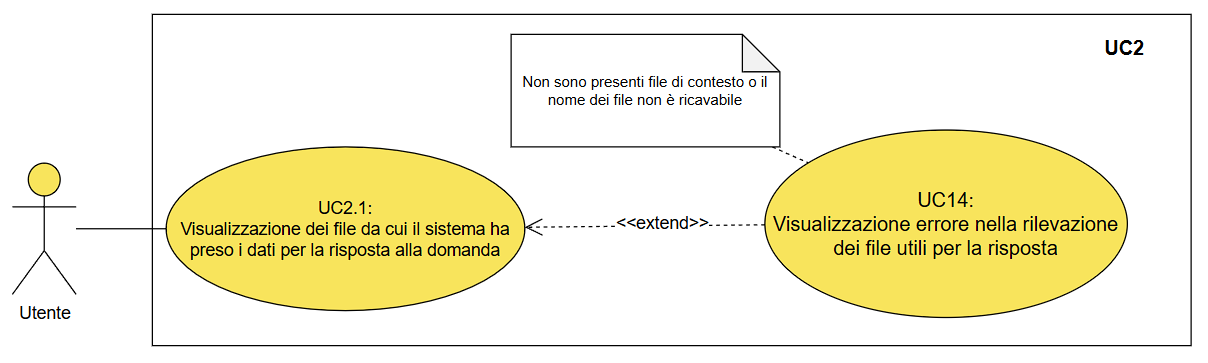
\includegraphics[width=\textwidth]{UC2.1+UC14.png}
    \caption{Visualizzazione dei file da cui il sistema ha preso i dati per la risposta alla domanda}
\end{figure}

\begin{itemize}
    \item \textbf{Attori principali}: Utente;
    \item \textbf{Precondizioni}: L'utente ha visualizzato la risposta generata;
    \item \textbf{Trigger}: L'utente desidera visualizzare i file da cui il sistema ha preso i dati per la risposta alla domanda;
    \item \textbf{Postcondizioni}: L'utente visualizza i file da cui il sistema ha preso i dati per la risposta alla domanda;
    \item \textbf{Scenario principale}:
    \begin{enumerate}
        \item L'utente accede all'interfaccia dell'applicazione;
        \item \bulhyperlink{UC1}{UC1}: L'utente inserisce un'interrogazione in linguaggio naturale;
        \item \bulhyperlink{UC2}{UC2}: L'utente visualizza la risposta generata;
        \item Il sistema rileva il file da cui ha generato la risposta;
        \item L'utente visualizza i file da cui il sistema ha preso i dati per la risposta alla domanda.
    \end{enumerate}
    \item \textbf{Scenario alternativo}:
    \begin{enumerate}
        \item \bulhyperlink{UC14}{UC14}: Visualizzazione errore nella rilevazione dei file utili per la risposta.
    \end{enumerate}
\end{itemize}

\hypertarget{UC14}{}
\subsubsection{UC14: Visualizzazione errore nella rilevazione dei file utili per la risposta}
\begin{itemize}
    \item \textbf{Attori principali}: Utente;
    \item \textbf{Precondizioni}: L'utente ha visualizzato la risposta generata;
    \item \textbf{Trigger}: L'utente desidera visualizzare i file da cui il sistema ha preso i dati per la risposta alla domanda;
    \item \textbf{Postcondizioni}: L'utente visualizza in fondo al messaggio di risposta una segnalazione di errore che comunica che non è stato possibile rilevare i file da cui è stata ricavata la risposta;
    \item \textbf{Scenario principale}: 
    \begin{enumerate}
        \item L'utente accede all'interfaccia dell'applicazione;
        \item \bulhyperlink{UC1}{UC1}: L'utente inserisce un'interrogazione in linguaggio naturale;
        \item \bulhyperlink{UC2}{UC2}: L'utente visualizza la risposta generata;
        \item Il sistema non riesce a rilevare i file da cui ha generato la risposta;
        \item L'utente visualizza in fondo al messaggio di risposta una segnalazione di errore che comunica che non è stato possibile rilevare i file da cui è stata ricavata la risposta.
    \end{enumerate}
\end{itemize}

\newpage

\hypertarget{UC6}{}
\subsubsection{UC6: Copia del testo della risposta generata}

\begin{figure}[h]
    \centering
    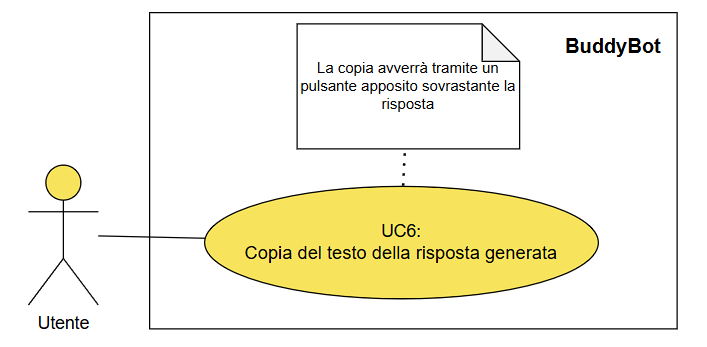
\includegraphics[width=\textwidth]{UC6.png}
    \caption{Copia del testo della risposta generata}
\end{figure}

\begin{itemize}
    \item \textbf{Attori principali}: Utente;
    \item \textbf{Precondizioni}: Il sistema ha generato una risposta valida e visibile alla domanda posta dall'utente;
    \item \textbf{Trigger}: L'utente desidera copiare il testo della risposta generata;
    \item \textbf{Postcondizioni}: Il testo della risposta generata viene copiato con successo nella clipboard del dispositivo e 
    diventa disponibile per l'uso da parte dell'utente in altre applicazioni o contesti;
    \item \textbf{Scenario principale}:
    \begin{enumerate}
        \item Il sistema ha generato correttamente la risposta alla domanda dell'utente;
        \item L'utente copia il testo della risposta generata premendo il pulsante che permette di copiarlo.
    \end{enumerate}
\end{itemize}


\hypertarget{UC7}{}
\subsubsubsection{UC7: Copia dello \emph{snippet} di codice inserito nella risposta}

\begin{figure}[h]
    \centering
    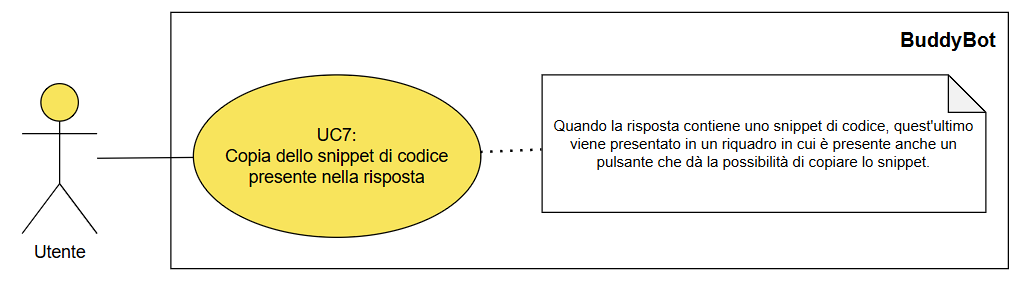
\includegraphics[width=\textwidth]{UC7.png}
    \caption{Copia dello \emph{snippet} di codice inserito nella risposta}
\end{figure}

\begin{itemize}
    \item \textbf{Attori principali}: Utente;
    \item \textbf{Precondizioni}: Il sistema ha generato una risposta valida con uno \emph{snippet} di codice al suo interno;
    \item \textbf{Trigger}: L'utente desidera copiare lo \emph{snippet} di codice inserito nella risposta;
    \item \textbf{Postcondizioni}: Lo \emph{snippet} di codice generato viene copiato con successo nella clipboard del dispositivo e diventa disponibile per l'uso da parte dell'utente in altre applicazioni o contesti;
    \item \textbf{Scenario principale}:
    \begin{enumerate}
        \item Il sistema ha generato correttamente la risposta alla domanda dell'utente con al suo interno dello \emph{snippet} di codice;
        \item L'utente copia lo \emph{snippet} di codice premendo il pulsante che permette di copiarlo.
    \end{enumerate}
\end{itemize}


\hypertarget{UC8}{}
\subsubsection{UC8: Visualizzazione dello storico della chat}

\begin{figure}[h]
    \centering
    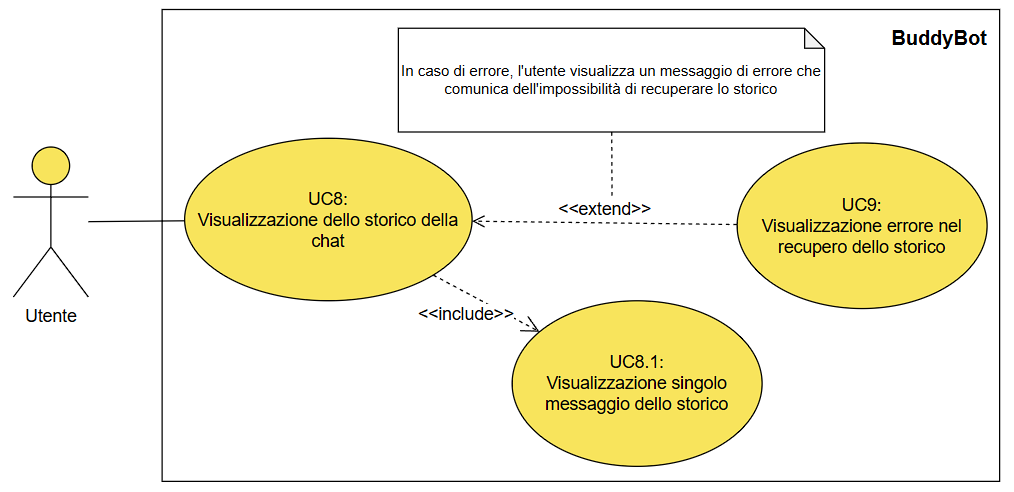
\includegraphics[width=\textwidth]{UC8+UC9.png}
    \caption{Visualizzazione dello storico della chat}
\end{figure}

\begin{itemize}
    \item \textbf{Attori principali}: Utente;
    \item \textbf{Precondizioni}: Il sistema deve essere collegato a un database relazionale per memorizzare e recuperare lo storico della chat;
    \item \textbf{Trigger}: L'utente desidera visualizzare lo storico della chat;
    \item \textbf{Postcondizioni}: L'utente visualizza lo storico della chat;
    \item \textbf{Scenario principale}:
    \begin{enumerate}
        \item L'utente avvia il sistema;
        \item Il sistema recupera i messaggi dello storico della chat dal database relazionale e li mostra a schermo;
        \item L'utente visualizza lo storico della chat.
    \end{enumerate}
    \item \textbf{Sottocasi d'uso}:
    \begin{itemize}
        \item \bulhyperlink{UC8.1}{UC8.1}: Visualizzazione singolo messaggio dello storico.
    \end{itemize}
    \item \textbf{Scenario alternativo}:
    \begin{enumerate}
        \item \bulhyperlink{UC9}{UC9}: Visualizzazione errore nel recupero dello storico.
    \end{enumerate}
\end{itemize}

\hypertarget{UC8.1}{}
\subsubsection{UC8.1: Visualizzazione singolo messaggio dello storico}
\begin{itemize}
    \item \textbf{Attori principali}: Utente;
    \item \textbf{Precondizioni}: Il sistema deve essere collegato a un database relazionale per memorizzare e recuperare lo storico della chat;
    \item \textbf{Trigger}: L'utente desidera visualizzare un singolo messaggio dello storico della chat;
    \item \textbf{Postcondizioni}: L'utente visualizza un singolo messaggio dello storico della chat;
    \item \textbf{Scenario principale}:
    \begin{enumerate}
        \item L'utente avvia il sistema;
        \item Il sistema recupera il messaggio dal database relazionale e lo mostra a schermo;
        \item L'utente visualizza il messaggio dello storico della chat.
    \end{enumerate}
\end{itemize}


\hypertarget{UC9}{}
\subsubsection{UC9: Visualizzazione errore nel recupero dello storico}
\begin{itemize}
    \item \textbf{Attori principali}: Utente;
    \item \textbf{Precondizioni}: Il sistema deve essere collegato a un database relazionale per memorizzare e recuperare lo storico della chat;
    \item \textbf{Trigger}: L'utente desidera visualizzare lo storico della chat;
    \item \textbf{Postcondizioni}: Viene visualizzato un messaggio di errore riferendo che c'è stato un errore nel recupero dello storico;
    \item \textbf{Scenario principale}: 
    \begin{enumerate}
        \item L'utente desidera visualizzare lo storico della chat;
        \item Il sistema ha riscontrato un problema nel recupero dello storico dal database relazionale;
        \item L'utente visualizza un messaggio di errore riferendo che c'è stato un errore nel recupero dello storico.
    \end{enumerate}
\end{itemize}


\hypertarget{UC10}{}
\subsubsection{UC10: Aggiornamento automatico del database vettoriale}

\begin{figure}[h]
    \centering
    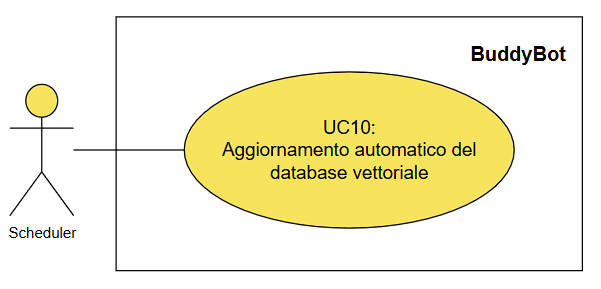
\includegraphics[width=\textwidth]{UC10.png}
    \caption{Aggiornamento automatico del database vettoriale}
\end{figure}

\begin{itemize}
    \item \textbf{Attori principali}: Scheduler;
    \item \textbf{Precondizioni}: 
    \begin{itemize}
        \item L'utente avvia l'applicazione;
        \item Il sistema è connesso al database vettoriale;
        \item Lo \emph{Scheduler} è attivo;
        \item E' arrivato il momento, prefissato dallo Scheduler, di aggiornare il database vettoriale.
    \end{itemize}
    \item \textbf{Trigger}: L'utente desidera ricevere risposte basate su dati aggiornati provenienti da \emph{GitHub}\textsubscript{\textbf{\textit{G}}}, 
    \emph{Jira}\textsubscript{\textbf{\textit{G}}} e \emph{Confluence}\textsubscript{\textbf{\textit{G}}};
    \item \textbf{Postcondizioni}: Lo scheduler ha aggiornato il database vettoriale con i dati più recenti provenienti da GitHub, Jira e Confluence;
    \item \textbf{Scenario principale}:
    \begin{enumerate}
        \item E' arrivato il momento, prefissato dallo Scheduler, di aggiornare il database vettoriale;
        \item Lo scheduler ha aggiornato il database vettoriale con i dati più recenti provenienti da GitHub, Jira e Confluence.
    \end{enumerate}
\end{itemize}


\hypertarget{UC11}{}
\subsubsection{UC11: Visualizzazione di una lista di domande ideali per iniziare la conversazione}

\begin{figure}[h]
    \centering
    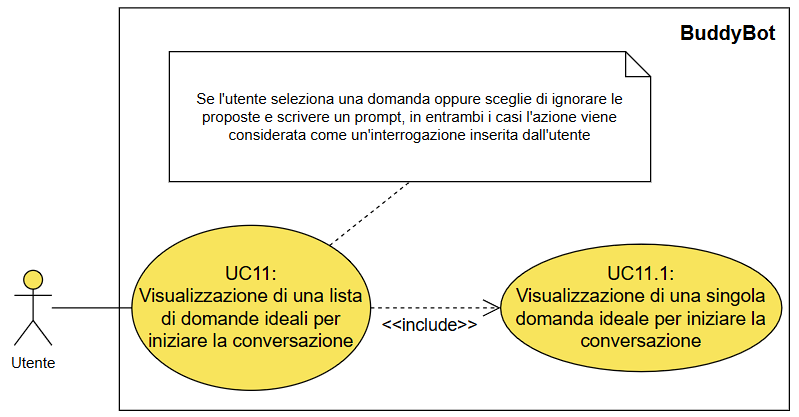
\includegraphics[width=\textwidth]{UC11.png}
    \caption{Visualizzazione di una lista di domande ideali per iniziare la conversazione}
\end{figure}

\begin{itemize}
    \item \textbf{Attori principali}: Utente;
    \item \textbf{Precondizioni}: L'utente ha appena cominciato una nuova conversazione;
    \item \textbf{Trigger}: L'utente desidera ricevere delle proposte di possibili domande per iniziare la conversazione;
    \item \textbf{Postcondizioni}: L'utente ha ricevuto una serie di domande suggerite dal sistema, che possono essere utilizzate per iniziare la conversazione;
    \item \textbf{Scenario principale}:
    \begin{enumerate}
        \item L'utente avvia l'applicazione;
        \item Il sistema propone una lista di domande ideali per iniziare la conversazione;
        \item \bulhyperlink{UC1}{UC1}: L'utente seleziona una delle domande proposte o inserisce una propria domanda.
    \end{enumerate}
    \item \textbf{Sottocasi d'uso}:
    \begin{itemize}
        \item \bulhyperlink{UC11.1}{UC11.1}: Visualizzazione di una singola domanda ideale per iniziare la conversazione;
    \end{itemize}
\end{itemize}

\hypertarget{UC11.1}{}
\subsubsection{UC11.1: Visualizzazione di una singola domanda ideale per iniziare la conversazione}
\begin{itemize}
    \item \textbf{Attori principali}: Utente;
    \item \textbf{Precondizioni}: L'utente ha appena cominciato una nuova conversazione;
    \item \textbf{Trigger}: L'utente desidera ricevere una proposta di domanda per iniziare la conversazione;
    \item \textbf{Postcondizioni}: L'utente visualizza una domanda suggerita dal sistema, che può essere utilizzata per iniziare la conversazione;
    \item \textbf{Scenario principale}:
    \begin{enumerate}
        \item L'utente avvia l'applicazione;
        \item Il sistema propone una domanda ideale;
        \item \bulhyperlink{UC1}{UC1}: L'utente seleziona la domanda proposta o inserisce una propria domanda.
    \end{enumerate}
\end{itemize}


\hypertarget{UC12}{}
\subsubsection{UC12: Visualizzazione di una lista di domande ideali per proseguire la conversazione}

\begin{figure}[h]
    \centering
    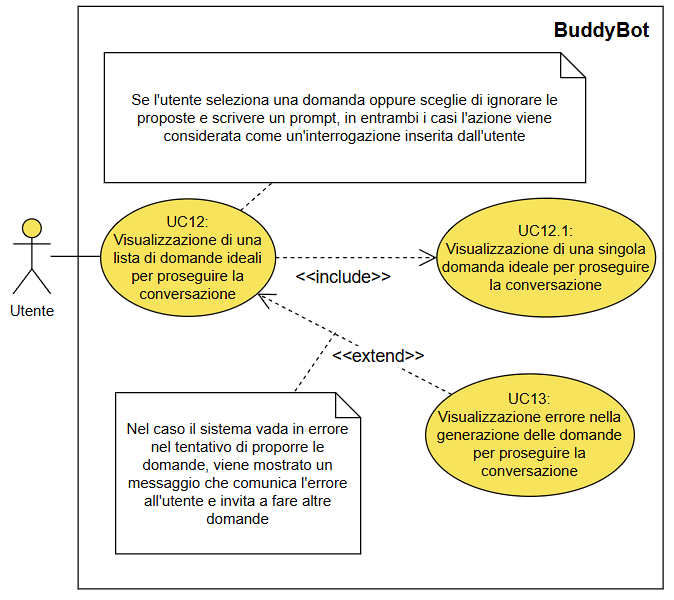
\includegraphics[width=\textwidth]{UC12+UC13.png}
    \caption{Visualizzazione di una lista di domande ideali per proseguire la conversazione}
\end{figure}

\begin{itemize}
    \item \textbf{Attori principali}: Utente;
    \item \textbf{Precondizioni}: L'utente ha appena ricevuto una risposta dal sistema;
    \item \textbf{Trigger}: L'utente desidera visualizzare delle proposte di possibili domande per proseguire la conversazione;
    \item \textbf{Postcondizioni}: L'utente visualizza una lista di domande suggerite dal sistema, che possono essere utilizzate per proseguire la conversazione;
    \item \textbf{Scenario principale}:
    \begin{enumerate}
        \item \bulhyperlink{UC2}{UC2}: L'utente ha visualizzato la risposta a una domanda precedente;
        \item Il sistema propone una lista di domande considerate utili rispetto ai messaggi precedenti;
        \item \bulhyperlink{UC1}{UC1}: L'utente seleziona una delle domande proposte o inserisce una propria domanda;
    \end{enumerate}
    \item \textbf{Sottocasi d'uso}:
    \begin{itemize}
        \item \bulhyperlink{UC12.1}{UC12.1}: Visualizzazione di una singola domanda ideale per proseguire la conversazione.
    \end{itemize}
    \item \textbf{Scenario alternativo}:
    \begin{enumerate}
        \item \bulhyperlink{UC13}{UC13}: Visualizzazione errore nella generazione delle domande per proseguire la conversazione.
    \end{enumerate}
\end{itemize}

\hypertarget{UC12.1}{}
\subsubsection{UC12.1: Visualizzazione di una singola domanda ideale per proseguire la conversazione}
\begin{itemize}
    \item \textbf{Attori principali}: Utente;
    \item \textbf{Precondizioni}: L'utente ha appena ricevuto una risposta dal sistema;
    \item \textbf{Trigger}: L'utente desidera visualizzare una proposta di domanda per proseguire la conversazione;
    \item \textbf{Postcondizioni}: L'utente visualizza una domanda suggerita dal sistema, che può essere utilizzata per proseguire la conversazione;
    \item \textbf{Scenario principale}:
    \begin{enumerate}
        \item \bulhyperlink{UC2}{UC2}: L'utente ha visualizzato la risposta a una domanda precedente;
        \item Il sistema propone una domanda ideale per proseguire la conversazione;
        \item L'utente visualizza la domanda proposta;
        \item \bulhyperlink{UC1}{UC1}: L'utente seleziona la domanda proposta o inserisce una propria domanda;
    \end{enumerate}
\end{itemize}

\hypertarget{UC13}{}
\subsubsection{UC13: Visualizzazione errore nella generazione delle domande per proseguire la conversazione}
\begin{itemize}
    \item \textbf{Attori principali}: Utente;
    \item \textbf{Precondizioni}: L'utente ha appena ricevuto una risposta dal sistema;
    \item \textbf{Trigger}: L'utente desidera visualizzare delle proposte di possibili domande per proseguire la conversazione;
    \item \textbf{Postcondizioni}: L'utente ha ricevuto un messaggio di errore che comunica che il sistema non è in grado di proporre delle domande;
    \item \textbf{Scenario principale}:
    \begin{enumerate}
        \item \bulhyperlink{UC2}{UC2}: L'utente ha visualizzato la risposta a una domanda precedente;
        \item Il sistema mostra un messaggio che comunica l'errore all'utente, e invita a fare altre domande.
    \end{enumerate}
\end{itemize}

\newpage

\hypertarget{UC15}{}
\subsubsection{UC15: Visualizzazione di un badge che segnala lo stato di aggiornamento del database vettoriale}

\begin{figure}[h]
    \centering
    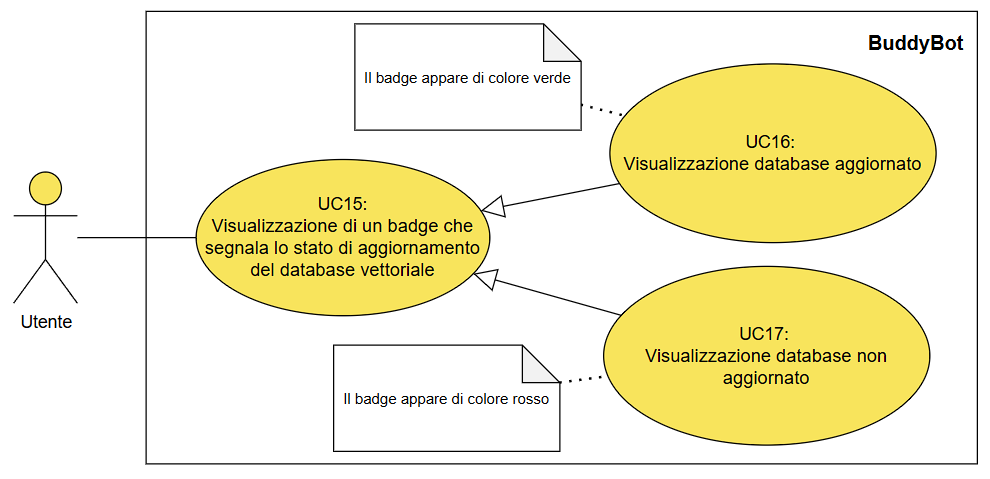
\includegraphics[width=\textwidth]{UC15+UC16+UC17.png}
    \caption{Visualizzazione di un badge che segnala lo stato di aggiornamento del database vettoriale}
\end{figure}

\begin{itemize}
    \item \textbf{Attori principali}: Utente;
    \item \textbf{Precondizioni}: L'utente avvia l'applicazione;
    \item \textbf{Trigger}: L'utente desidera verificare se il database vettoriale è stato aggiornato;
    \item \textbf{Postcondizioni}: L'utente visualizza un badge che segnala lo stato di aggiornamento del database vettoriale;
    \item \textbf{Scenario principale}:
    \begin{enumerate}
        \item L'utente avvia l'applicazione;
        \item Il sistema segnala lo stato di aggiornamento del database vettoriale.
    \end{enumerate}
    \item \textbf{Casi che ereditano}:
    \begin{itemize}
        \item \bulhyperlink{UC16}{UC16}: Visualizzazione database aggiornato;
        \item \bulhyperlink{UC17}{UC17}: Visualizzazione database non aggiornato.
    \end{itemize}
\end{itemize}

\hypertarget{UC16}{}
\subsubsection{UC16: Visualizzazione database aggiornato}
\begin{itemize}
    \item \textbf{Attori principali}: Utente;
    \item \textbf{Precondizioni}: L'utente avvia l'applicazione;
    \item \textbf{Trigger}: L'utente desidera verificare se il database vettoriale è stato aggiornato;
    \item \textbf{Postcondizioni}: L'utente visualizza un badge indicativo che il database vettoriale è aggiornato;
    \item \textbf{Scenario principale}:
    \begin{enumerate}
        \item L'utente avvia l'applicazione;
        \item Il sistema segnala che il database vettoriale è aggiornato tramite un badge di colore verde.
    \end{enumerate}
    \item \textbf{Eredita da}:
    \begin{itemize}
        \item \bulhyperlink{UC15}{UC15}: Visualizzazione di un badge che segnala lo stato di aggiornamento del database vettoriale.
    \end{itemize}
\end{itemize}

\hypertarget{UC17}{}
\subsubsection{UC17: Visualizzazione database non aggiornato}
\begin{itemize}
    \item \textbf{Attori principali}: Utente;
    \item \textbf{Precondizioni}: L'utente avvia l'applicazione;
    \item \textbf{Trigger}: L'utente desidera verificare se il database vettoriale è stato aggiornato;
    \item \textbf{Postcondizioni}: L'utente visualizza un badge indicativo che il database vettoriale non è aggiornato;
    \item \textbf{Scenario principale}:
    \begin{enumerate}
        \item L'utente avvia l'applicazione;
        \item Il sistema segnala che il database vettoriale non è aggiornato tramite un badge di colore rosso.
    \end{enumerate}
    \item \textbf{Eredita da}:
    \begin{itemize}
        \item \bulhyperlink{UC15}{UC15}: Visualizzazione di un badge che segnala lo stato di aggiornamento del database vettoriale.
    \end{itemize}
\end{itemize}